\documentclass[11pt, compress]{beamer}

\usetheme{m}

\usepackage{booktabs}
\usepackage[scale=2]{ccicons}
\usepackage{minted}
\usepackage[binary-units=true]{siunitx}
\usepackage{caption}
\usepackage{subcaption}

\usemintedstyle{trac}

\title{Big Data Random Forests in R}
\subtitle{}
\date{April 2016}
\author{Andrew Nisbet}
\institute{MSA220 project 1}

\begin{document}


\maketitle

  \setbeamercolor{background canvas}{bg=white}
\begin{frame}[fragile]
  \frametitle{Project}

  \textbf{Aim: } investigate using R to perform random forest classification on a large dataset.
  
  \begin{itemize}
      \item Predict delays from flight information
      \item Compare \texttt{randomForest} and \texttt{bigrf}
      \item Evaluate performance
  \end{itemize}
  
  
\end{frame}

\begin{frame}[fragile]
  \frametitle{Overview}


  \begin{itemize}
      \item About big data
      \item Dataset creation
      \item \texttt{randomForest}
      \item \texttt{bigrf}
      \item Conclusion
  \end{itemize}
  
  
\end{frame}

\begin{frame}[fragile]
  \frametitle{Big Data - RAM}

  Keep everything in RAM, otherwise use disk intelligently.
  
  \begin{table}[h!]
\centering
\begin{tabular}{ l c c }
  \toprule
  & Hard Drive & RAM\\
  \midrule
  Transfer Rate & \SI{50}{\mega\byte\per\second} & \SI{5000}{\mega\byte\per\second} \\
  Access Delay & \SI{10000000}{\nano\second} & \SI{10}{\nano\second}  \\
  \bottomrule
\end{tabular}
\end{table}
\end{frame}

\begin{frame}[fragile]
  \frametitle{Big Data - Motivation}
\begin{figure}[ht]
  \centering
  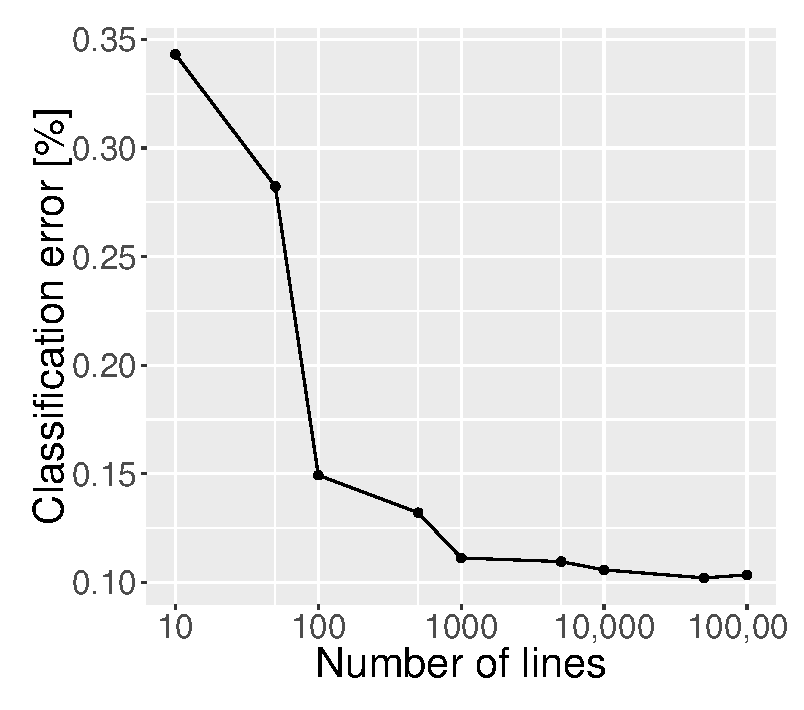
\includegraphics[height=7cm]{rf_error.eps}
%   \caption{\label{rf_error} Validation error rate for subsets of different sizes.}
\end{figure}
\end{frame}

\begin{frame}[fragile]
  \frametitle{Dataset - Overview}

  \begin{itemize}
    \item Combination of flight (\SI{12}{\giga\byte}) and weather (\SI{3}{\giga\byte}) data.
    \item Fight features
    \begin{minted}[fontsize=\small]{latex}
        Day of the week, duration, airport
    \end{minted}
    \item Weather features
    \item Only flights leaving a single airport
    \item $y$ = whether flight was delayed
    \item Final dataset had \SI{5000000}{lines}, 19 features, \SI{500}{\mega\byte}
    \item big-$n$
\end{itemize}
\end{frame}

\begin{frame}[fragile]
  \frametitle{Dataset - Subsetting}
    Large datasets distrup standard workflows. Methods to create a \SI{5000000}{line} subset:
  \begin{itemize}
    \item \texttt{read.table}: crashed
    \item \texttt{read.table}: \SI{250}{\second}
    \begin{itemize}
        \item Read column types in advance
        \item Specify \texttt{nrows} (from \texttt{wc -l input.csv})
    \end{itemize}
    \item \texttt{fread}: \SI{20}{\second} (\texttt{data.table})
    \item \texttt{shuf}: \SI{2}{\second} (Linux command line)
    \begin{minted}[fontsize=\small]{latex}
        shuf -n 10000 input.csv > output.csv
    \end{minted}

\end{itemize}
\end{frame}

\begin{frame}[fragile]
  \frametitle{\texttt{randomForest} - Overview}
  
  
  
    Most common package
  \begin{itemize}
    \item Limited to 53 factor levels
    \item Single process
\end{itemize}
\end{frame}

\begin{frame}[fragile]
  \frametitle{\texttt{randomForest} - Results}
  \begin{figure}[ht]
    \begin{subfigure}[t]{0.49\textwidth}
        \centering
        \includegraphics[height=4.5cm]{rf_time.eps}
        % \caption{Forest build time.}
    \end{subfigure}%
    \begin{subfigure}[t]{0.49\textwidth}
        \centering
        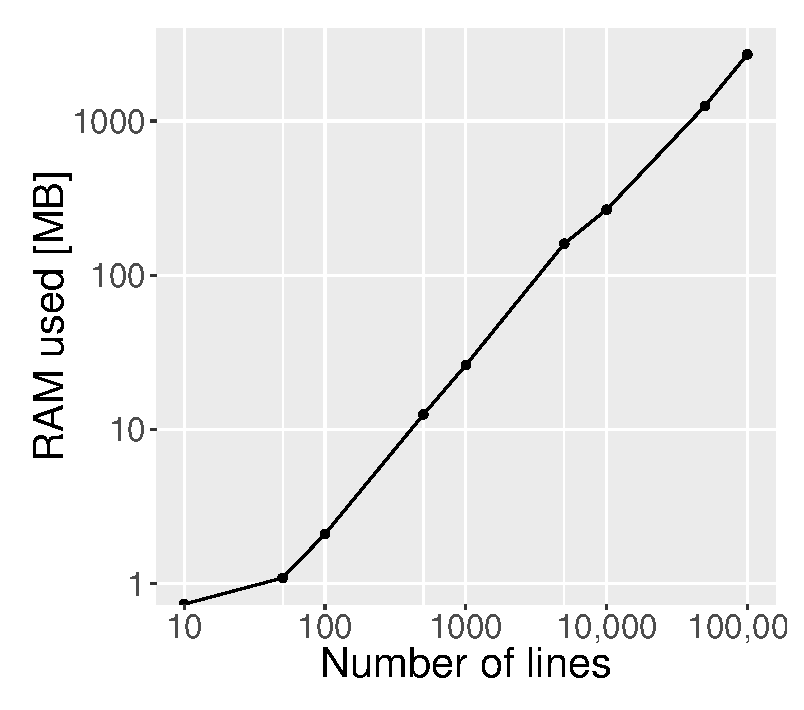
\includegraphics[height=4.5cm]{rf_ram.eps}
        % \caption{Total RAM usage, including data and forest.}
    \end{subfigure}
    % \caption{\label{rf} \texttt{randomForest} results for different subsets.}
\end{figure}

    Crashed after \SI{100000}{lines}.
  
 
\end{frame}

\begin{frame}[fragile]
  \frametitle{\texttt{bigrf} - Overview}
    

  \begin{itemize}
    \item Uses \texttt{big.matrix} for data and trees
    \item Data shared between processes
    \item Data can be saved to disk and queried
    \item Outputs useful statistics
    \item Linux/OSX only
    \item Lack of support and documentation
\end{itemize}
\end{frame}

\begin{frame}[fragile]
  \frametitle{\texttt{bigrf} - Results}
  \begin{figure}[ht]
    \begin{subfigure}[t]{0.49\textwidth}
        \centering
        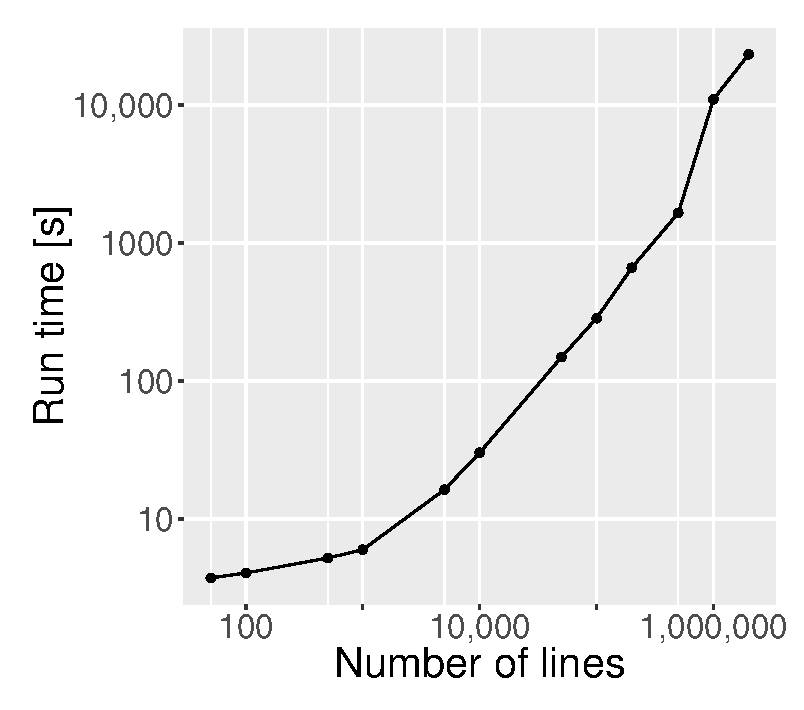
\includegraphics[height=4.5cm]{bigrf_time.eps}
        % \caption{Forest build time.}
    \end{subfigure}%
    \begin{subfigure}[t]{0.49\textwidth}
        \centering
        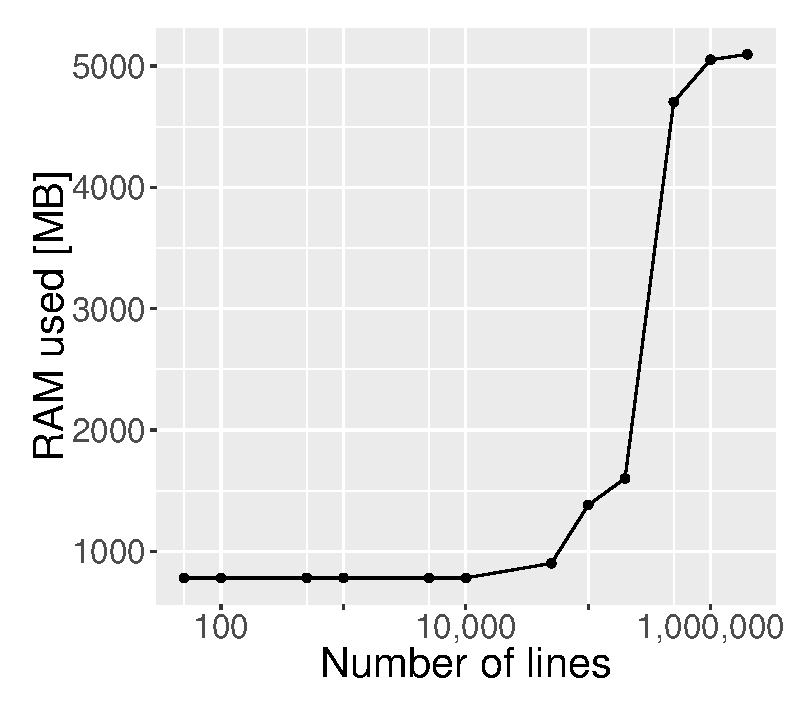
\includegraphics[height=4.5cm]{bigrf_ram.eps}
        % \caption{Total RAM usage, including data and forest.}
    \end{subfigure}
    % \caption{\label{rf} \texttt{randomForest} results for different subsets.}
\end{figure}

    Crashed after \SI{2000000}{lines}.
  
 
\end{frame}

\begin{frame}[fragile]
  \frametitle{Conclusion}

  \begin{itemize}
    \item R can be used for large datasets, just choose the right tools
    \item \texttt{bigrf} is nice to work with, compared to \texttt{randomForest}
    \item \texttt{bigrf} can handle much larger datasets without crashing, but performs poorly for small datasets
\end{itemize}
\end{frame}


\plain{}{Questions?}

\end{document}
